\documentclass[11pt,a4paper]{article}
\usepackage[hyperref]{conll-2019}
\usepackage{amsmath, amssymb, amsthm, amscd, amsfonts}
\usepackage{times}
\usepackage{latexsym}
\usepackage{graphicx}
\usepackage{epstopdf}
\usepackage{algorithm}
\usepackage{algorithmicx}
\usepackage{algpseudocode}
\usepackage{url}
\usepackage{subfigure}
\usepackage[UTF8]{ctex}
\usepackage{enumerate}
\usepackage{multirow}
\usepackage[OT1]{fontenc}



\aclfinalcopy

\newcommand\confname{CoNLL 2019}
\newcommand\conforg{SIGNLL}
\newcommand\BibTeX{B\textsc{ib}\TeX}
\renewcommand{\algorithmicrequire}{ \textbf{Input:}}
\renewcommand{\algorithmicensure}{ \textbf{Output:}}

\newcommand{\tabincell}[2]{\begin{tabular}{@{}#1@{}}#2\end{tabular}}
\newcommand{\toprightarrow}[1]{\mathord{\buildrel{\lower3pt\hbox{$\scriptscriptstyle\rightarrow$}}\over#1} }
\newcommand{\topleftarrow}[1]{\mathord{\buildrel{\lower3pt\hbox{$\scriptscriptstyle\leftarrow$}}\over#1} }



\title{KDABert: Knowledge Distillation with Generative Adversarial Networks for Bert Model Compression}

\author{闫森\\
  \texttt{2017111497} \\}

\date{}

\begin{document}
\maketitle
\begin{abstract}
    这里是摘要。这里是摘要。这里是摘要。这里是摘要。这里是摘要。这里是摘要。这里是摘要。
    这里是摘要。这里是摘要。这里是摘要。这里是摘要。这里是摘要。这里是摘要。这里是摘要。
\end{abstract}

\section{介绍}
\label{Sec:Introduction}
这里是介绍。这里是介绍。这里是介绍。这里是介绍。这里是介绍。这里是介绍。这里是介绍。
这里是介绍。这里是介绍。这里是介绍。这里是介绍。这里是介绍。这里是介绍。这里是介绍。

\begin{figure}[htbp]
    \centering
    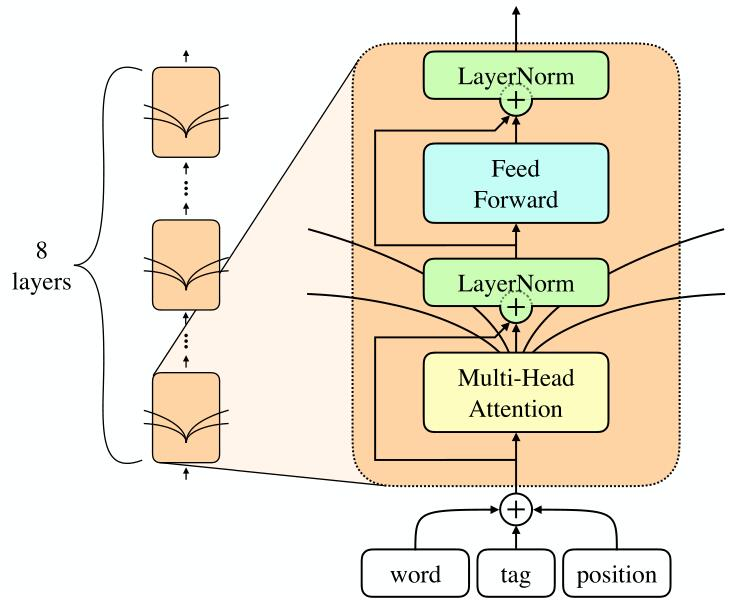
\includegraphics[width=\linewidth]{images/multi_headed_attention.jpg}
    \caption{Transformer结构。}
    \label{Fig:multi_headed_attention}
\end{figure}

\section{实验}
这里是实验。这里是实验。这里是实验。这里是实验。这里是实验。这里是实验。这里是实验。
这里是实验。这里是实验。这里是实验。这里是实验。这里是实验。这里是实验。这里是实验。
这里是实验。这里是实验。这里是实验。这里是实验。这里是实验。这里是实验。这里是实验。
这里是实验。这里是实验。这里是实验。这里是实验。这里是实验。这里是实验。这里是实验。
这里是实验。这里是实验。这里是实验。这里是实验。这里是实验。这里是实验。这里是实验。
\begin{table}[htbp]
    \normalsize
    \begin{center}
        \begin{tabular}{l|ccc}
            \hline
            模型                                     & LR   & LP   & F1            \\
            \hline
            \textbf{单模型}                                                         \\
            \hline
            \citet{DBLP:conf/nips/VinyalsKKPSH15}     & -    & -    & 88.3          \\
            \citet{DBLP:conf/naacl/DyerKBS16}         & -    & -    & 89.8          \\
            \citet{DBLP:conf/acl/ZhuZCZZ13}           & 90.2 & 90.7 & 90.4          \\
            \citet{DBLP:conf/emnlp/CrossH16}          & 90.5 & 92.1 & 91.3          \\
            \citet{DBLP:journals/tacl/LiuZ17}         & 91.3 & 92.1 & 91.7          \\
            \citet{DBLP:conf/acl/SternAK17}           & 90.3 & 93.2 & 91.8          \\
            \citet{DBLP:journals/tacl/LiuZ17a}        & -    & -    & 91.8          \\
            \citet{DBLP:conf/acl/BengioSCJLS18}       & 92.0 & 91.7 & 91.8          \\
            \citet{DBLP:conf/acl/HongH18}             & 91.5 & 92.5 & 92.0          \\
            \citet{DBLP:conf/coling/TengZ18}          & 92.2 & 92.5 & 92.4          \\
            \citet{DBLP:conf/emnlp/SternFK17}         & 92.5 & 92.5 & 92.5          \\
            \citet{DBLP:conf/acl/KleinK18}            & 93.2 & 93.9 & \textbf{93.6} \\
            \hline\hline
            \textbf{非单模型}                                         \\
            \hline
            \citet{DBLP:conf/emnlp/ChoeC16}           & -    & -    & 93.8          \\
            \citet{DBLP:journals/tacl/LiuZ17a}        & -    & -    & 94.2          \\
            \citet{DBLP:conf/acl/FriedSK17}           & -    & -    & 94.7          \\
            \citet{DBLP:conf/acl/KleinK18}            & 94.9 & 95.4 & 95.1          \\
            \citet{DBLP:journals/corr/abs-1812-11760} & 95.6 & 96.0 & \textbf{95.8} \\
            \hline
        \end{tabular}
    \end{center}
    \caption{不同模型在PTB测试集上的最终结果。}
    \label{Tab:FinalResults}
\end{table}


\section*{致谢}
这里是致谢。这里是致谢。这里是致谢。这里是致谢。这里是致谢。这里是致谢。这里是致谢。
这里是致谢。这里是致谢。这里是致谢。这里是致谢。这里是致谢。这里是致谢。这里是致谢。

\newpage
\bibliography{conll-2019}
\bibliographystyle{acl_natbib}

\end{document}
